\section{Packaging} \label{sec:packaging}

%\begin{minipage}{.7\textwidth}
\begin{itemize}
    \item Wire bonding 
	\begin{itemize}
	    \item max. $\diameter 1\un{mil} \,\,(\approx 25\un{\mu m})$\footnote{CRESSTO s.r.o., Rožnov p. R., \url{www.cressto.cz}}\footnote{SEANT Technology s.r.o., Brno, \url{www.seant.cz}} contrary to $15\un{mil}$ used for IGBTs
	    \item max. continuous current $\approx 1\un{A/1wire}$; 8 wires tested as sufficient for double pulse current over $80\un{A}$
	\end{itemize}
    \item encapsulation: epoxy resin - availability and simple treatment
	\begin{itemize}
	    \item dilatation harmless even for bond wires of $\diameter 1\un{mil}$
	\end{itemize}
\end{itemize}
%\end{minipage}

%\begin{minipage}{.3\textwidth}
\begin{figure}[!ht]
    \centering
    \vspace{.3\textheight}
    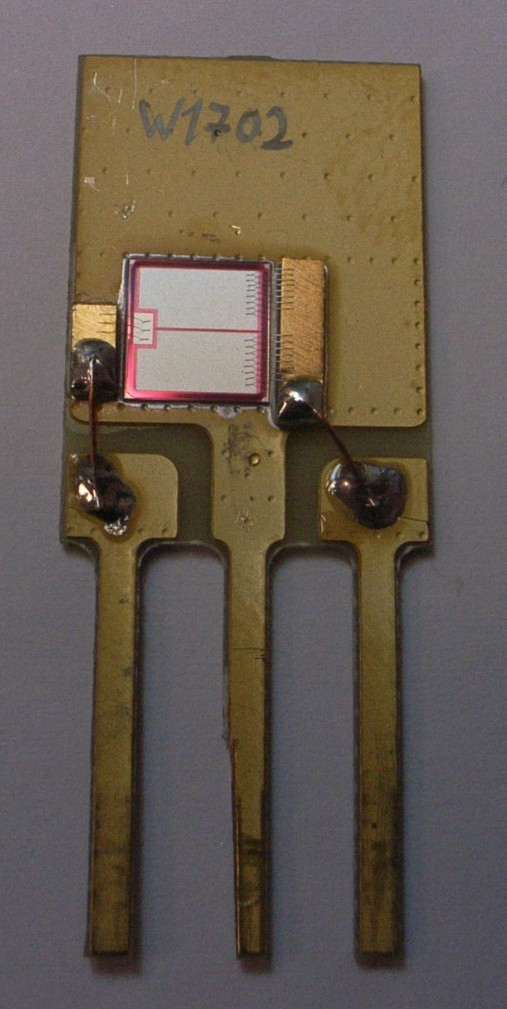
\includegraphics[height=.4\textheight]{pkg_be}
    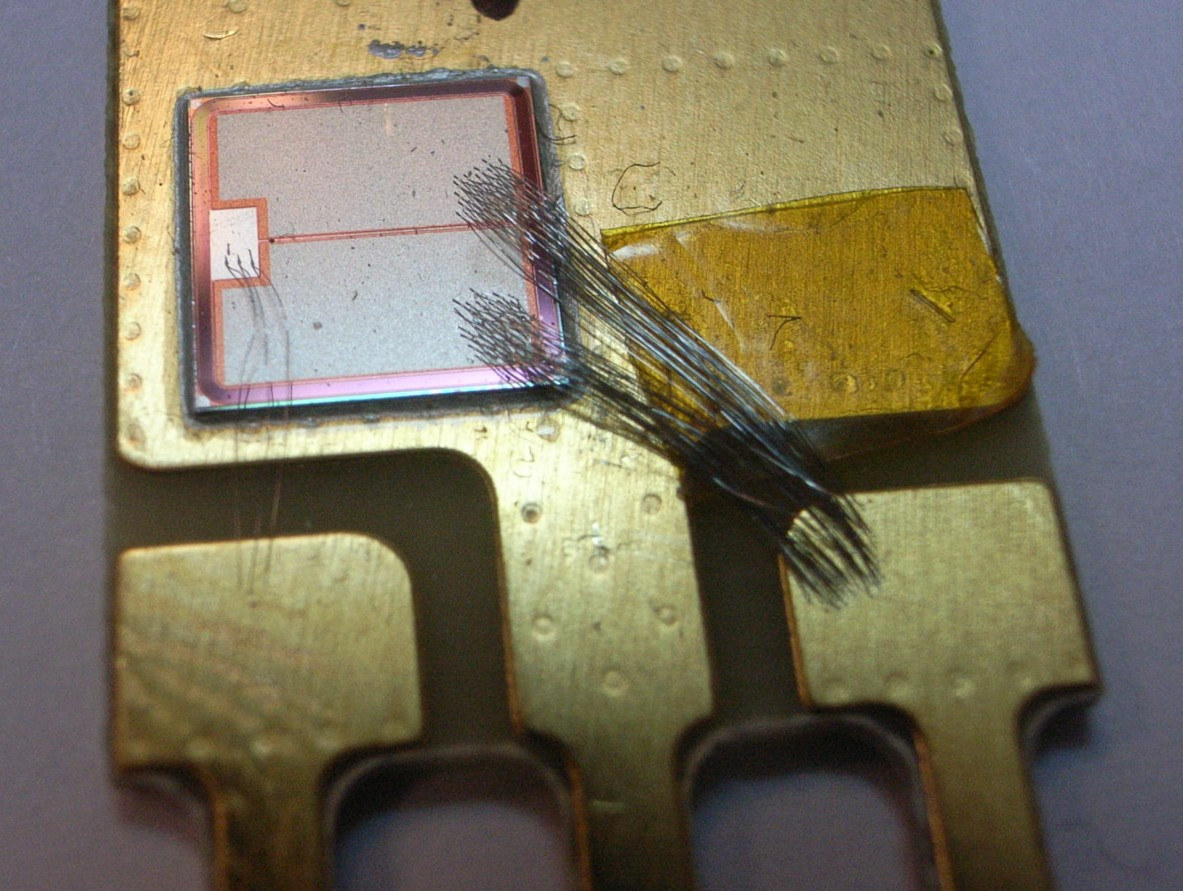
\includegraphics[height=.4\textheight]{bond1}
    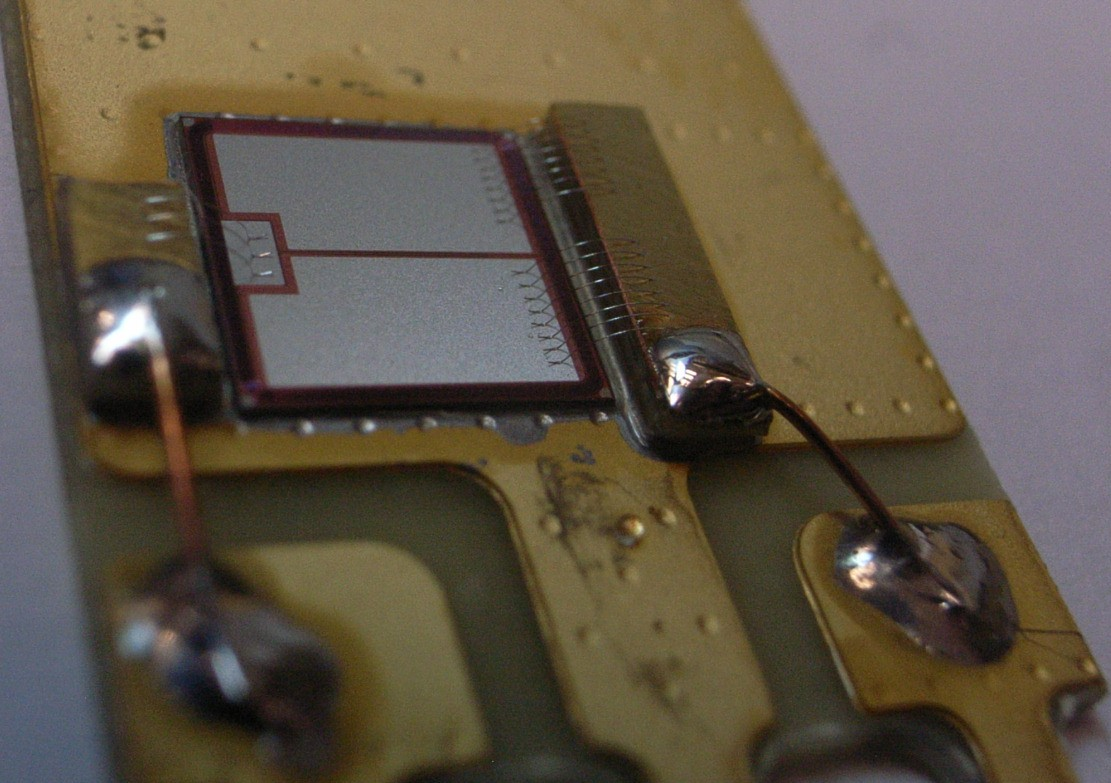
\includegraphics[height=.4\textheight]{bond2}
    \caption{``TO247'' package before epoxy encapsulation.}
    \label{fig:pkg_be}
\end{figure}
%\end{minipage}
